
\documentclass[twoside,onecolumn]{article}

\usepackage{blindtext} % Package to generate dummy text throughout this template 

%\usepackage[sc]{mathpazo} % Use the Palatino font
\usepackage[T1]{fontenc} % Use 8-bit encoding that has 256 glyphs
\linespread{1.05} % Line spacing - Palatino needs more space between lines
\usepackage{microtype} % Slightly tweak font spacing for aesthetics
\usepackage{float}
 \usepackage{amsmath}
 \usepackage{booktabs}
 \usepackage{amssymb}
 \usepackage{amsthm}
 \usepackage{tabularx} %tabelle
 \usepackage{tikz} %circuiti
 \usepackage{enumerate}
 \usepackage{pgfplots}
 \usepackage{subcaption}
\usepackage[toc,page]{appendix}
 \usepackage[export]{adjustbox}
 \usepackage{caption}
 \usepackage{subfig}
 \usepackage{sidecap}
 \usepackage{graphicx}
 \theoremstyle{definition}
  \usepackage{multicol}
  \usetikzlibrary{arrows}
  \usepackage[shortlabels]{enumitem}

\usepackage[english]{babel} % Language hyphenation and typographical rules

\usepackage[hmarginratio=1:1,top=32mm,columnsep=20pt]{geometry} % Document margins
\usepackage[hang, small,labelfont=bf,up,textfont=it,up]{caption} % Custom captions under/above floats in tables or figures
\usepackage{booktabs} % Horizontal rules in tables
\usepackage[square,numbers]{natbib}
\bibliographystyle{unsrtnat}
\usepackage{lettrine} % The lettrine is the first enlarged letter at the beginning of the text

\usepackage{enumitem} % Customized lists
\setlist[itemize]{noitemsep} % Make itemize lists more compact

\usepackage{titlesec} % Allows customization of titles
\titleformat{\section}[block]{\large\scshape\centering}{\thesection.}{1em}{} % Change the look of the section titles
\titleformat{\subsection}[block]{\large}{\thesubsection.}{1em}{} % Change the look of the section titles

\usepackage{hyperref} % For hyperlinks in the PDF

\title{Homework 3: Simulations} % Article title
\author{Nicole Zattarin}
\date{} 
\begin{document}

% Print the title
\maketitle

\begin{abstract}
ciao belli

\end{abstract}

\section{Single service queue}
Let us consider a single server queue, we perform a discrete-time simulation under the assumption that arrivals cannot leave in the same slot in which they arrive. We consider the following situations:
\begin{enumerate}[(a)]
\item $P[\text{1 arrival}]=P[\text{2 arrivals}]=a, P[\text{0 arrival}]=1-2a$, $a\in [0,0.5].$ and single service time for each user;
\item $P[\text{1 arrival}]=P[\text{0 arrival}]=0.5$ and geometric service time with mean probability $b$. 
\end{enumerate}
We design a program that simulate a fixed number of time slots (10000 in our case) and computes the average throughput, delay, occupancy, arrival rate, service time and returns the whole history of the queue state. Moreover, we are interested in studying the stability of the queue, to do so we compute the utilization factor $\rho$, which is computed as follows:
\begin{equation}
\rho = \frac{\text{average arrival rate}}{\text{average service time}}.
\end{equation}
From the previous definition it is pretty intuitive to understand that the condition for stability is the following:
\begin{itemize}
\item $\rho>1$ the rate of arrivals cannot be compensated with the departure rate, i.e. service time is too long to serve enough users and the state diverges;
\item $\rho=1$ the rate of arrivals is equal to the service time, thus we would expect to observe the queue periodically getting empty for a while, but after a certain time it is likely that the status diverges.
\item $\rho<1$ the service time is such that it is possibile to serve all users, thus the queue periodically empties because users arrived are quickly served.
\end{itemize}
Finally, to make our simulation more realistic, we implement a finite-size buffer system, such that if a new arrival would exceed the maximum queue size, it is dropped. This mechanism also allows to measure the overflow probability of a queueing system.

\subsection{Single service time - 0/1/2 arrivals}
In case (a) the average service time is constant, thus the value of $\rho$ depends on the arrivals rate: the more is the probability of observing 1 or 2 arrivals the larger will be $\rho$:  $\rho\propto a$ . 
Indeed, in Figure \ref{fig:rho_fixedtime} we show delay, i.e. the time a user waits in the queue until it can be served, vs  $\rho$ by varying a from 0 to 1/3. We can observe that $\rho$ grows with the delay, while both delay and $\rho$ increase with $a$ .As we already pointed out, we would have expected to observe $\rho$ increasing with $a$, since larger values of $a$ correspond to a higher probability of observing 1 and 2 arrivals with respect to 0 arrivals. Moreover, delay increases with $\rho$ since higher values of $\rho$, in the case of a fixed service time, correspond to an accumulation of users in the queue that are waiting to be served.
\par
In Figure \ref{fig:fixedtime_state} we show the realization of queue size vs time for 10000 slots. Figure   \ref{fig:fixedtime_state_stable} shows results for $a=1/4$, which corresponds to $\rho = 0.77$, thus to a stable queue. We can observe the expected behaviour for a stable system: the queue periodically empties, then new users are added and so on for a theoretically infinite time. On the other hand, figure \ref{fig:fixedtime_state_critical} exhibits the same plot for $a=1/3$, $\rho = 1$. In this case the behaviour is less stable, the queue status oscillates and the system empties once, but the general trend is increasing. Finally,  Figure \ref{fig:fixedtime_state_critical} shows the unstable simulation for $a=1/2$, $\rho = 1.5$, in this case the probability of observing zero arrivals is null, while service time is still fixed to 1. As a consequence the number of users waiting to be served diverges. 

\begin{figure} \centering
         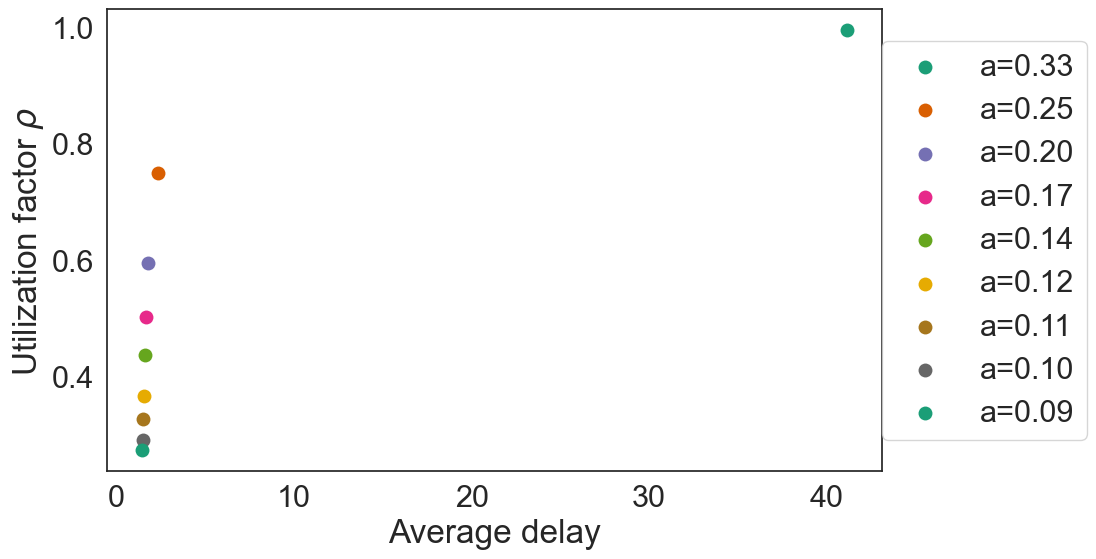
\includegraphics[width=0.7\textwidth]{../single_server_queue/figures/delay_vs_rho_fixedtime.png}
    \caption{Queueing system with  $P[\text{1 arrival}]=P[\text{2 arrivals}]=a, P[\text{0 arrival}]=1-2a$ and unitary service time, delay vs  $\rho$ by varying a from 0 to 1/3.  }\label{fig:rho_fixedtime}
\end{figure}


\begin{figure} \centering
\begin{subfigure}{\textwidth}
         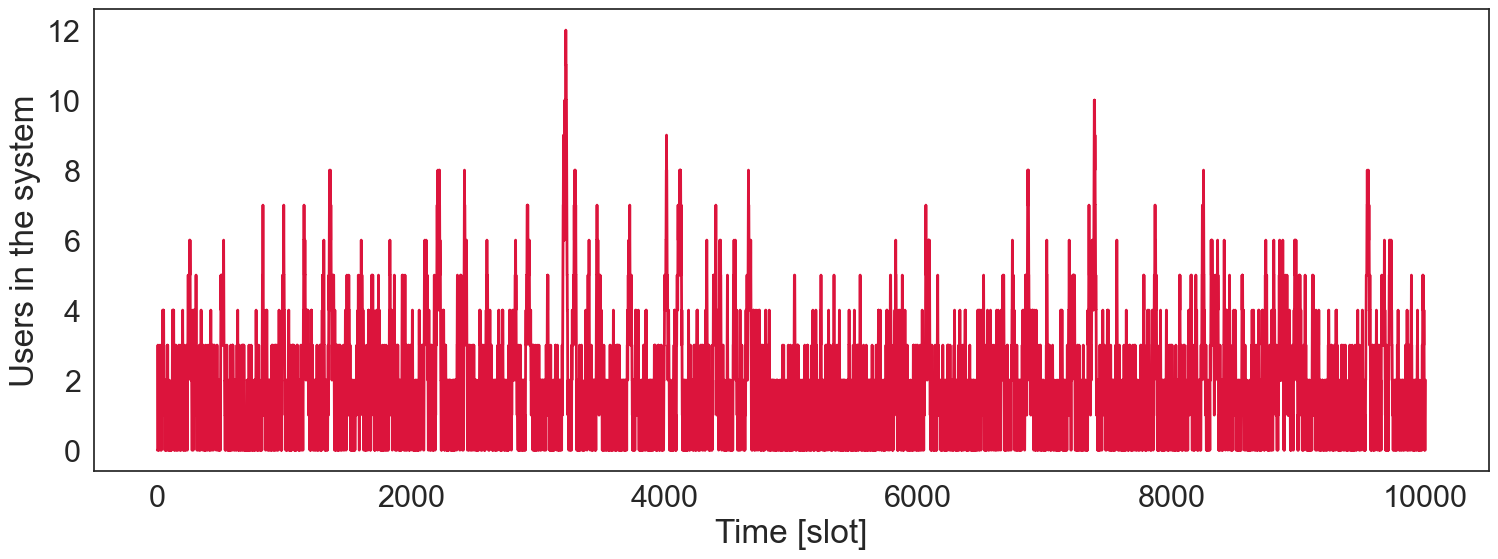
\includegraphics[width=\textwidth]{../single_server_queue/figures/queue_size_vs_time_a=0.25.png}
         \caption{Queue size for a stable queueing system, P[\text{1 arrival}]=P[\text{2 arrivals}]=0.25, P[\text{0 arrival}]=0.5$, $\rho=0.77$.}\label{fig:fixedtime_state_stable}
     \end{subfigure}
     
     \begin{subfigure}{\textwidth}
         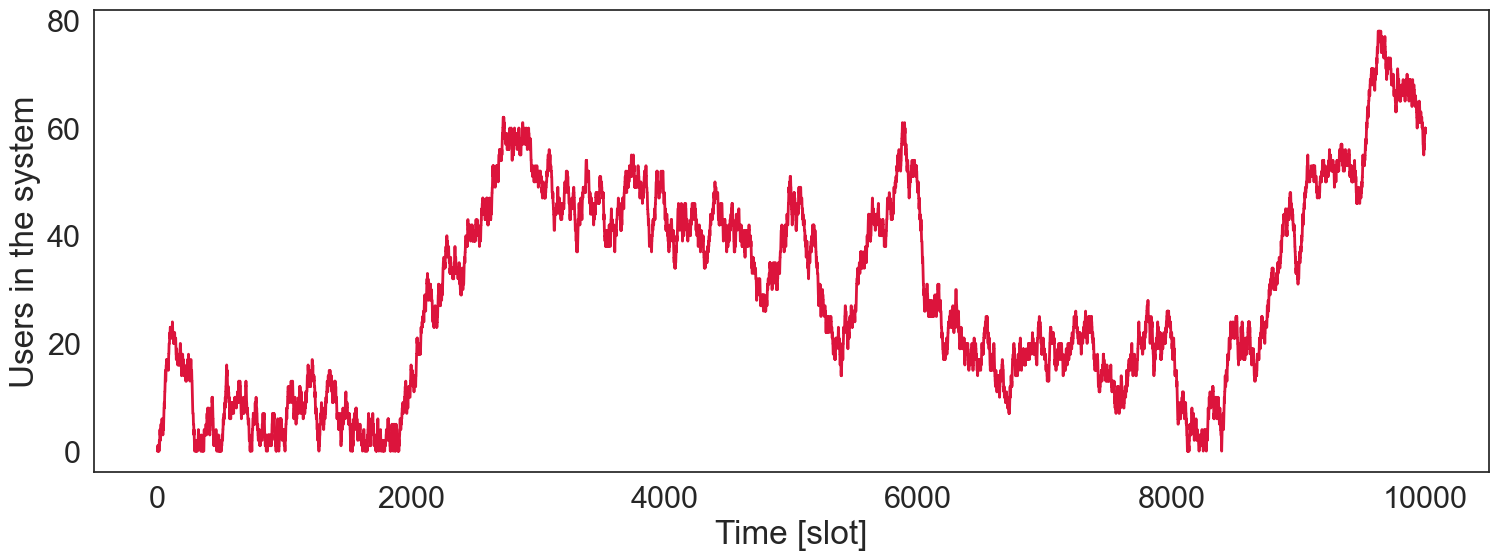
\includegraphics[width=\textwidth]{../single_server_queue/figures/queue_size_vs_time_a=0.33.png}
         \caption{Queue size for a critical queueing system, P[\text{1 arrival}]=P[\text{2 arrivals}]=0.33, P[\text{0 arrival}]=0.33$, $\rho=1$.}\label{fig:fixedtime_state_critical}
     \end{subfigure}
     
          \begin{subfigure}{\textwidth}
         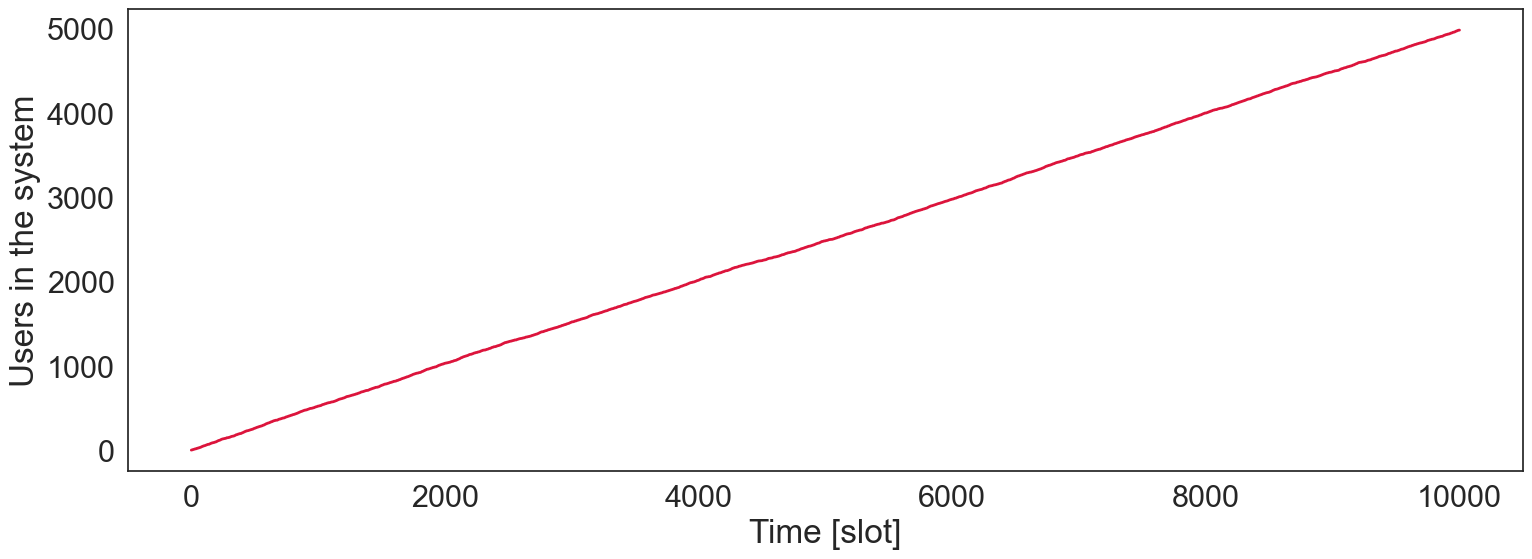
\includegraphics[width=\textwidth]{../single_server_queue/figures/queue_size_vs_time_a=0.50.png}

         \caption{Queue size for an unstable queueing system, P[\text{1 arrival}]=P[\text{2 arrivals}]=0.50, P[\text{0 arrival}]=0$, $\rho=1.5$.}\label{fig:fixedtime_state_unstable}
     \end{subfigure}
     
  \caption{Realization of queue size vs time for 10000 slots for different values of 1 and 2 arrivals probabilities, fixed service time.   }\label{fig:fixedtime_state}
\end{figure}


\subsection{Geometric service time - 0/1 arrivals }
In case (b) the average service time is a geometric RV with mean value $1/b$, as a consequence the value of $\rho$ depends on the parameter $b$. In this case we would expect the opposite behaviour: larger values of $b$ correspond to larger faster service time in average and then to a faster processing of users in the queue.  

In Figure \ref{fig:geo_state} we show delay vs  $\rho$ by varying $b$ from 0.5 to 1, as already introduced we observe that $\rho$ grows with delay, while both delay and $\rho$ decrease with $b$. Thus, in this case jobs are processed faster and users wait for less time in queue as $b$ increases.
\par
In Figure \ref{fig:geo_state} we show the realization of queue size vs time for 10000 slots. Figure \ref{fig:geo_state_unstable} shows results for $b=1/3$ and $\rho = 1.50$, in Figure \ref{fig:geo_state_critical} we have $b=1/2$ and $\rho = 1$, and  n Figure \ref{fig:geo_state_stable} we have $b=2/3$ and $\rho = 0.77$. In a completely analogous way as in case (a), but with the opposite trend, the previous cited figures denote respectively a non-stable, critical and stable queueing system.

\begin{figure} \centering
         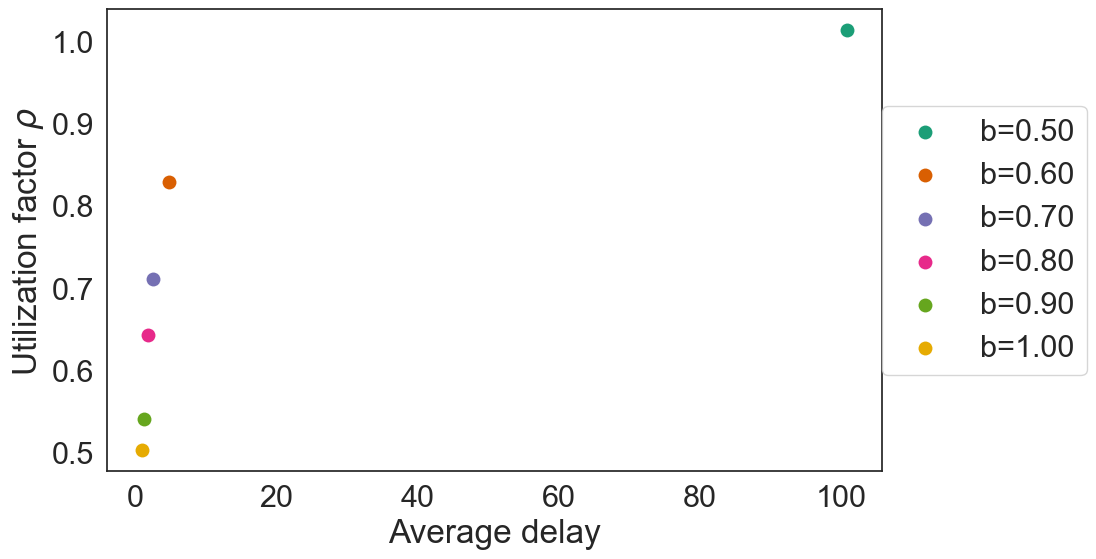
\includegraphics[width=0.7 \textwidth]{../single_server_queue/figures/delay_vs_rho_geometric.png}
    \caption{Queueing system with fixed 0 and 1 user arrivals probabilities and geometric service times with probability $b$, delay vs $\rho$ by varying $b$ from 0.5 to 1 }\label{fig:}
\end{figure}

\begin{figure} \centering
\begin{subfigure}{\textwidth}
         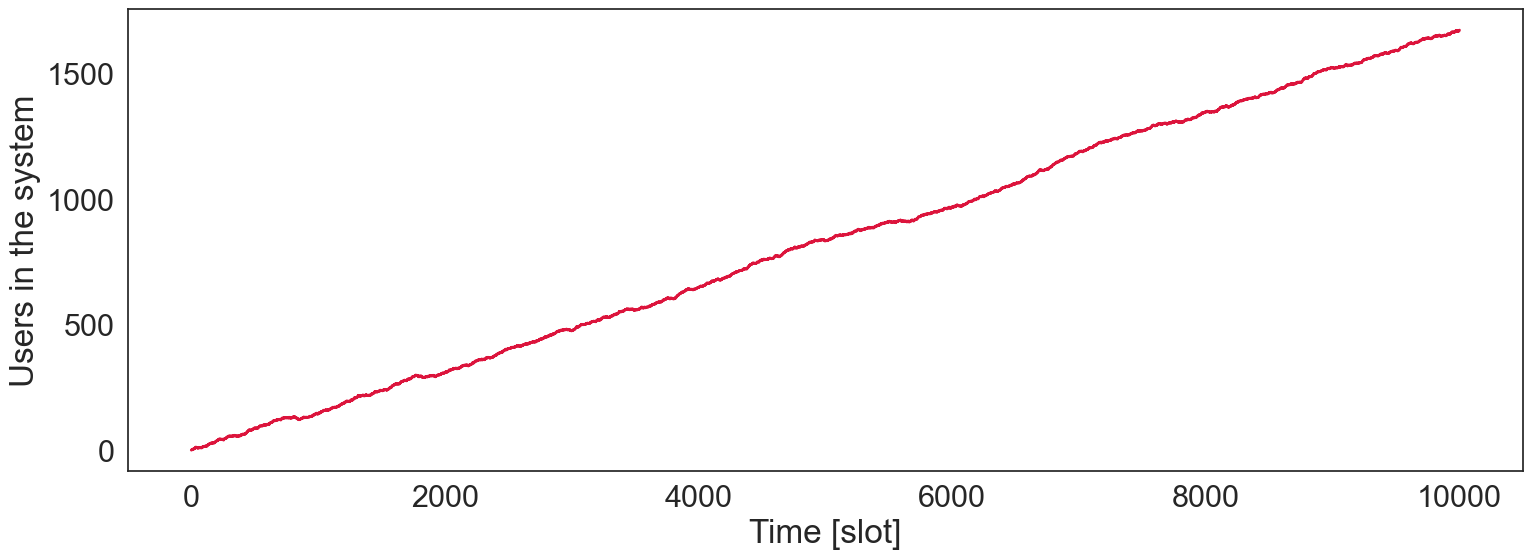
\includegraphics[width=\textwidth]{../single_server_queue/figures/queue_size_vs_time_b=0.33.png}
         \caption{Queue size for an unstable queueing system, P[\text{1 arrival}]=P[\text{0 arrivals}]=0.5, $b=0.33$, \rho=1.5$.}\label{fig:geo_state_unstable}
     \end{subfigure}
     
     \begin{subfigure}{\textwidth}
         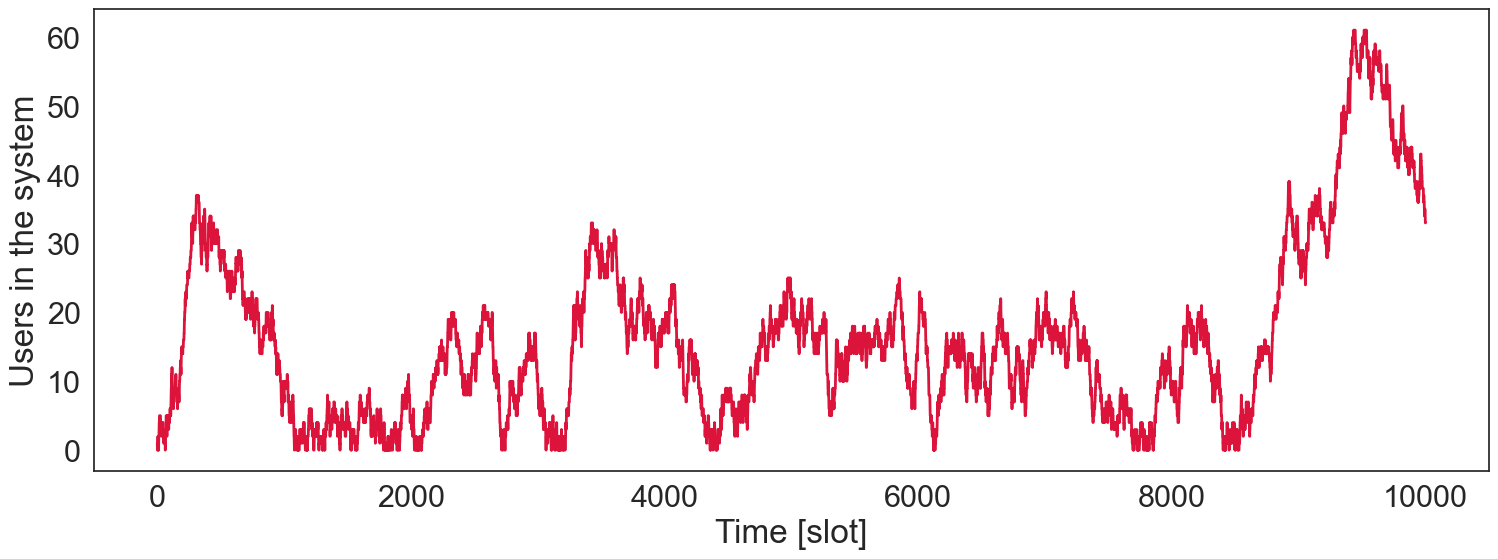
\includegraphics[width=\textwidth]{../single_server_queue/figures/queue_size_vs_time_b=0.50.png}
         \caption{Queue size for a critical queueing system, P[\text{1 arrival}]=P[\text{0 arrivals}]=0.5, $b=0.5$, \rho=1$.}\label{fig:geo_state_critical}
     \end{subfigure}
     
          \begin{subfigure}{\textwidth}
         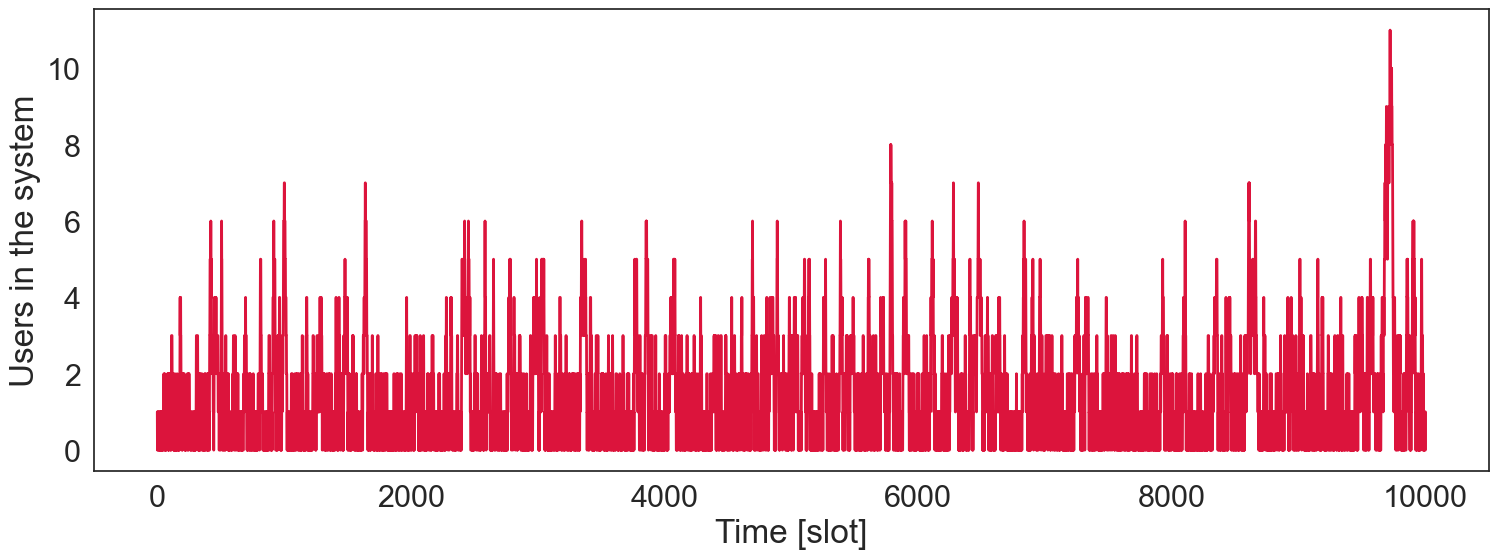
\includegraphics[width=\textwidth]{../single_server_queue/figures/queue_size_vs_time_b=0.67.png}

         \caption{Queue size for a stable queueing system, P[\text{1 arrival}]=P[\text{0 arrivals}]=0.5, $b=0.67$, \rho=0.77$.}\label{fig:geo_state_stable}
     \end{subfigure}
     
  \caption{Realization of queue size vs time for 10000 slots for fixed values of 1 and 0 arrivals probabilities, geometric service times with different probabilities. }\label{fig:geo_state}
\end{figure}

\subsection{Overflow probability}
As we already pointed out, the service system is such that if the a new arrival would exceed the buffer size it is dropped. Before computing explicitly the buffer sizes necessary to guarantee a certain dropping probability, let us have a further look at Figures \ref{fig:geo_state_stable} and \ref{fig:fixedtime_state_stable}. It is worth to highlight that the number of users in the system is constantly lower than 12 and, apart from a few isolated points, it is in general lower than 8.  

We now want to be quantitative and perform a bisection root search to find the \textit{integer} value of buffer size which guarantees a probability $0.001\%$ of overflow, results for the cases $\rho\leq1$ are reported in Table \ref{tab:overflow}. The main outcome is that stable queues don't need a huge buffer capacity to provide a low dropping probability, while as the behaviour becomes more critical a larger queue is required. Finally, note also that results are similar, if not the same, for both simulations. This is not surprising, since the overflow probability depends on the nature of the system, if it is stable or not, so on the value of $\rho$, independently of the system employed to manage the queueing system.

\begin{table}\centering
\begin{tabular}{c|c|c|c}
Case&Parameter     &  $\rho$   & Buffer size for $0.001\%$ overflow \\ \hline
(b) & b=2/3& $ 0.77$ & 8                                  \\
(b) & b=1/2 &$ 1$    & 79                                 \\
(a) & a=1/4& $ 0.77$ & 8                                \\
(a) & a=1/3&$ 1$    & 73                                
\end{tabular}        \caption{Values of buffer sizes which guarantee a probability $0.001\%$ of overflow for different stable simulations. }\label{tab:overflow}
\end{table}


\section{SINR performance}
A useful quantity to measure the quality of a signal is the SINR (Signal to Interference and Noise Ratio), which basically takes into account the strength of the wanted signal compared to the unwanted interference and noise. Given a communication system affected by noise and interference, we want to evaluate its performances in terms of probability to correctly deliver the information, to do so, we compute the probability that the SNR is greater than a fixed threshold $b$:
\begin{equation}\label{eq:ps}
P_s=P[SNR>b],
\end{equation}
where we refer to $b$ also as capture ratio. Moreover, $P_s$ can be computed analytically as follows:
\begin{equation}\begin{split}\label{eq:integral}
P_s(r_0)& = \int_{-\infty}^{+\infty}\frac{d\xi_0}{\sqrt{2\pi}\sigma}e^{-\frac{\xi_0^2}{2\sigma^2}}[I(\xi_0,r_0)]^k,\\
I(\xi_0,r_0)&=\int_{-\infty}^{+\infty}\frac{d\xi}{\sqrt{2\pi}\sigma}e^{-\frac{\xi^2}{2\sigma^2}}\int_0^1\frac{h(r)dr}{1+be^{\xi-\xi_0}(\frac{r}{r_0})^{-\eta}},
\end{split}\end{equation}
where $\xi_0$ is normally distributed with zero mean and $\sigma^2$ variance, $r_0$ is the position of the intended user and $r$ is distributed as the interferers.
To solve the problem, i.e. to find Equation \ref{eq:ps}, two possible approaches are computationally feasible: 
\begin{itemize}
\item Montecarlo simulation: randomly generate multiple times the involved variables with the required statistic and compute the frequency of the event $SNR>b$;
\item  Gauss Quadrature Rules to compute the integral in Equation \ref{eq:integral}.
\end{itemize}
The system described is still generic and can be used to describe different physical systems, we study the following situation:
\begin{itemize}
\item Packet radio: we compute the capture probabilities , $r_0$ is fixed, while $r$ is in $[0,\infty)$;
\item Cellular systems: we are interested in computing the outrage probability, $r_0$ uniform in the cell, while $r$ follows the distribution of interferers;
\item ALOHA: we compute throughput, all users in the same area, all r in [0,1].
\end{itemize}

\subsection{Packet radio}
\begin{figure} \centering
         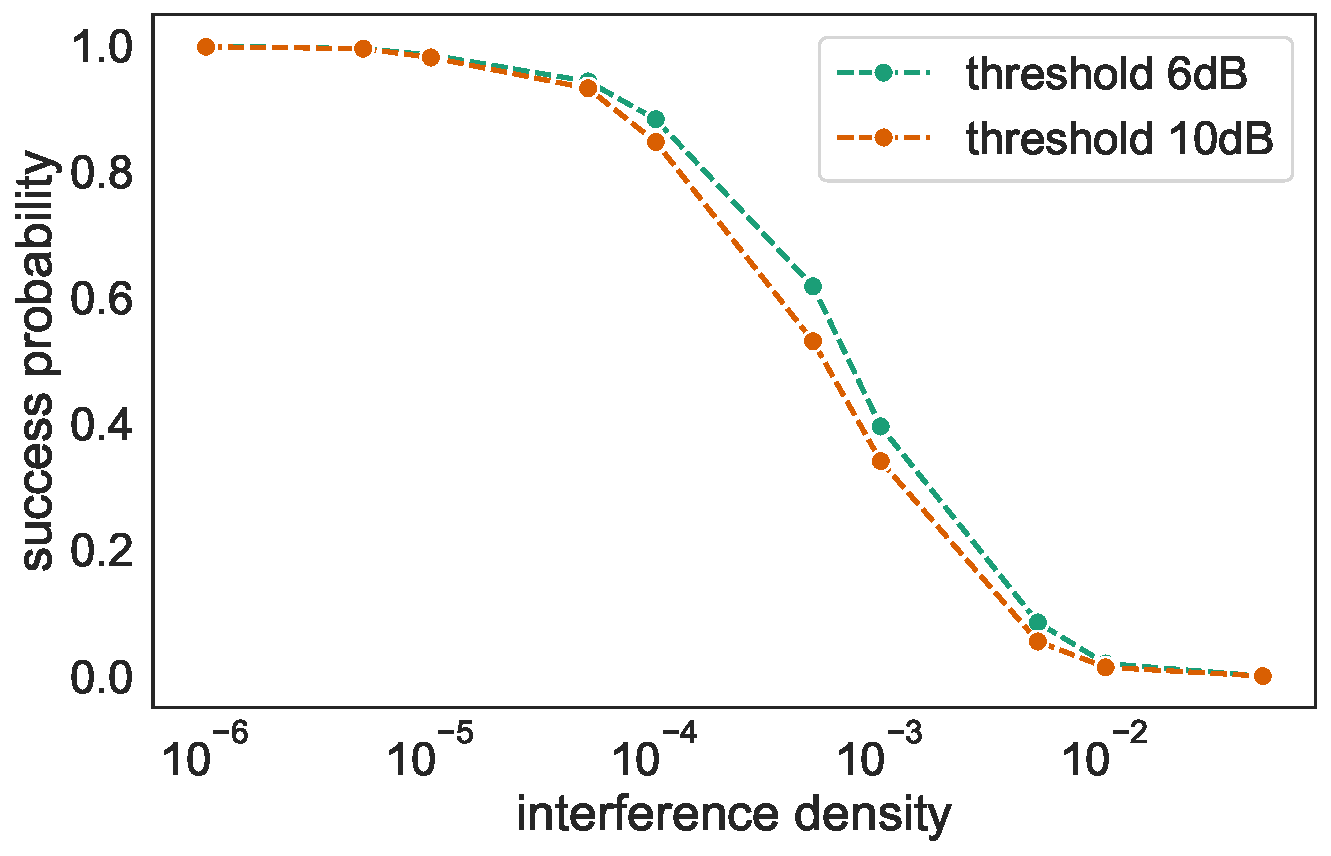
\includegraphics[width=0.65\textwidth]{../SINR_systems/figures/packet_radio.pdf}
    \caption{ }\label{fig:}
\end{figure}

\subsection{Cellular systems}
\begin{figure} \centering
         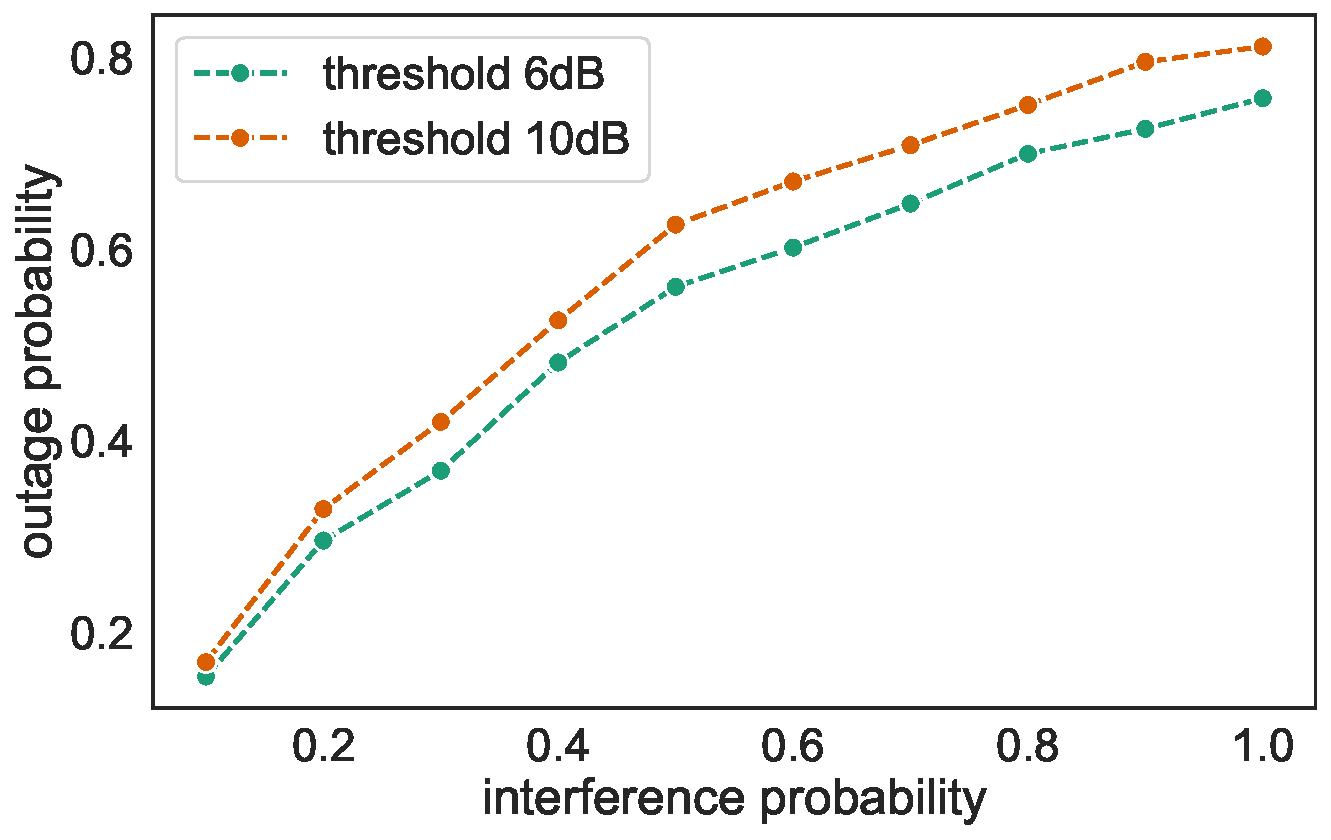
\includegraphics[width=0.65\textwidth]{../SINR_systems/figures/cellular_system.pdf}
    \caption{ }\label{fig:}
\end{figure}

\subsection{ALOHA}
\begin{figure} \centering
         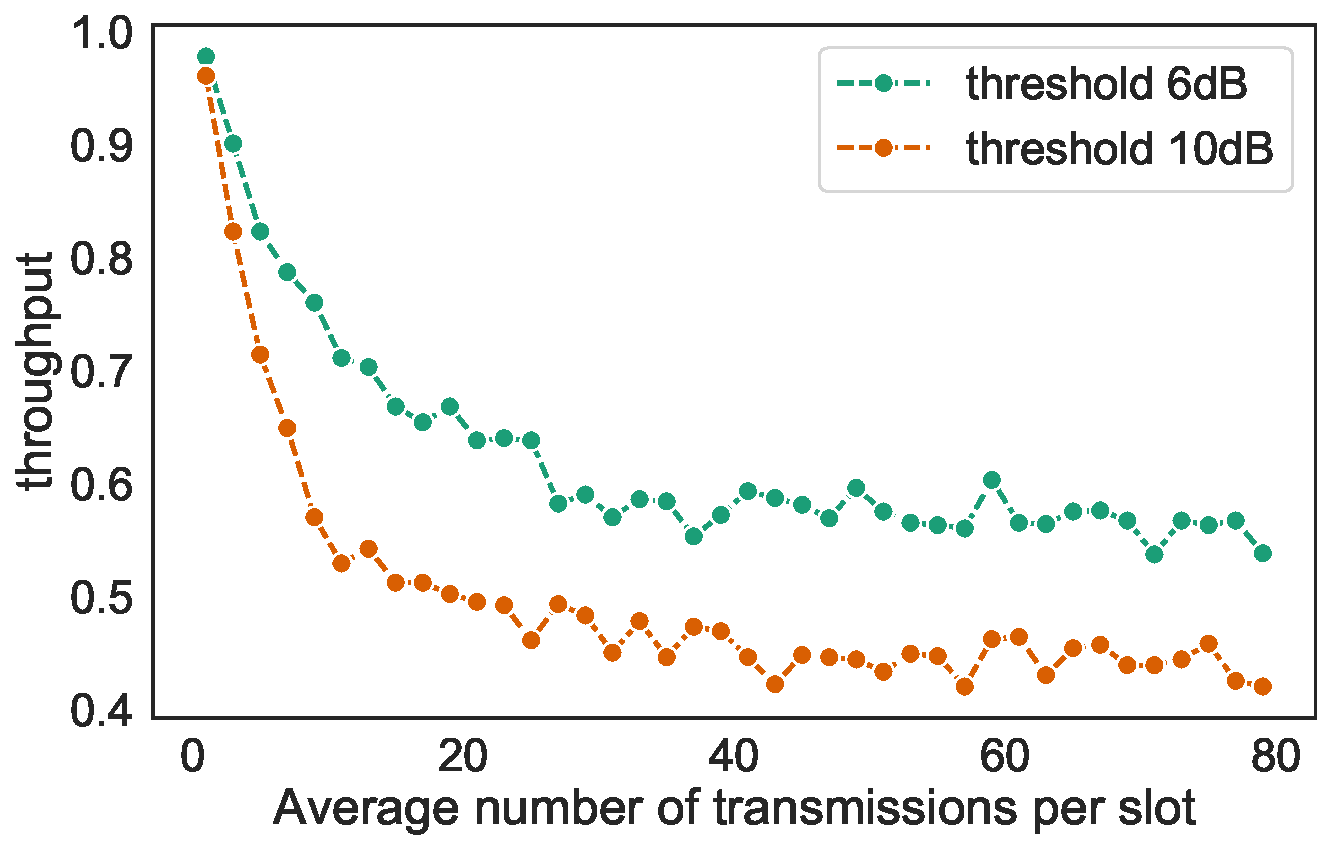
\includegraphics[width=0.65\textwidth]{../SINR_systems/figures/multi_access.pdf}
    \caption{ }\label{fig:}
\end{figure}

\section{GeRaF multihop performance}
In this section we reproduce the results proposed in \cite{zorzi2}  and compare the Geographic Random Forwarding (GeRaF) model performances with GAF \cite{gaf}, see also \cite{zorzi1} for further analysis.
In particular, we implement GeRaF algorithm for the estimation of the average number of hops needed per the forwarding. In Figure \ref{fig:gaf} we exhibit the average number of hops  with the respective standard deviations vs average number of active nodes for different distances, averages are computed over a sample of 100 simulations results. In particular, we can observe that GeRaF performs better than GAF best case for a reasonable number of active nodes. Moreover, the number of hops quickly decreases up to about 10 nodes and then almost get stabilized on a value which depends on the distance, but that is still better than GAF in any case.

\begin{figure} \centering
\begin{subfigure}{0.45\textwidth}
         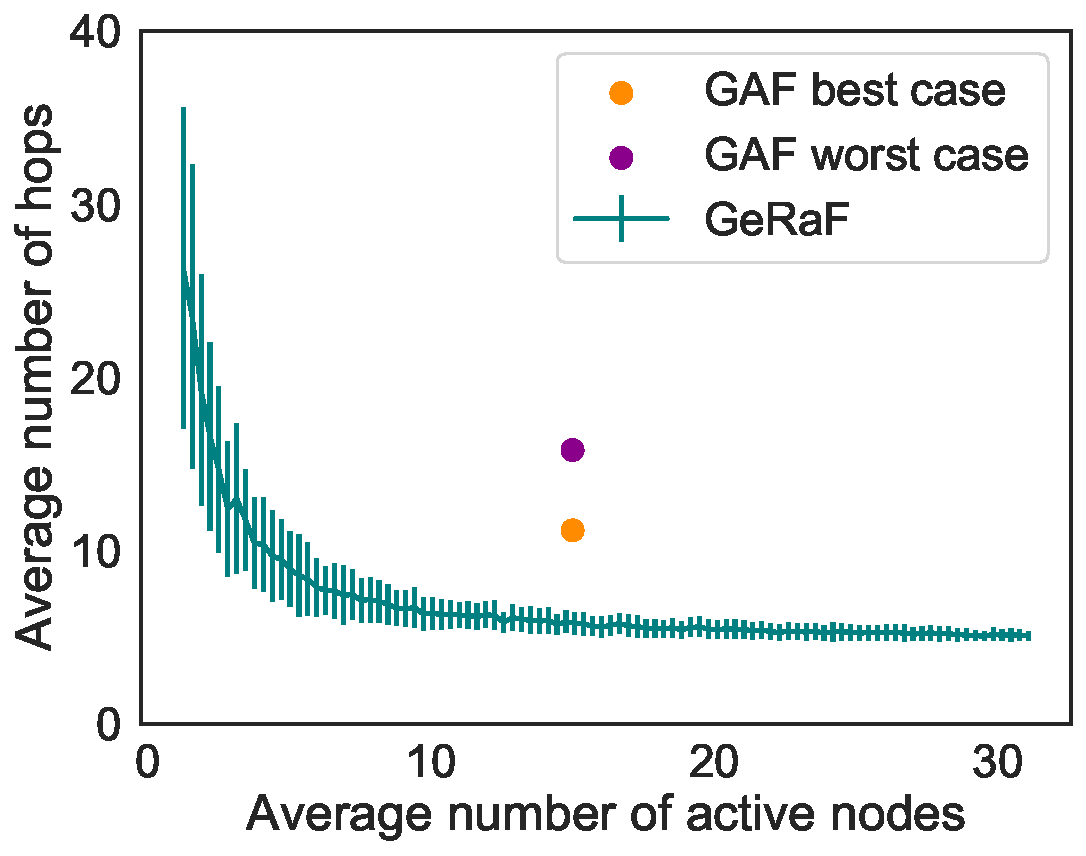
\includegraphics[width=\textwidth]{../multihop_GeRaF/figures/multihop_GeRaF_N100_distance5.pdf}
         \caption{Average number of hops vs average number of active nodes for $D=5$.}\label{fig:gaf5}
     \end{subfigure}
     \quad
     \begin{subfigure}{0.45\textwidth}
         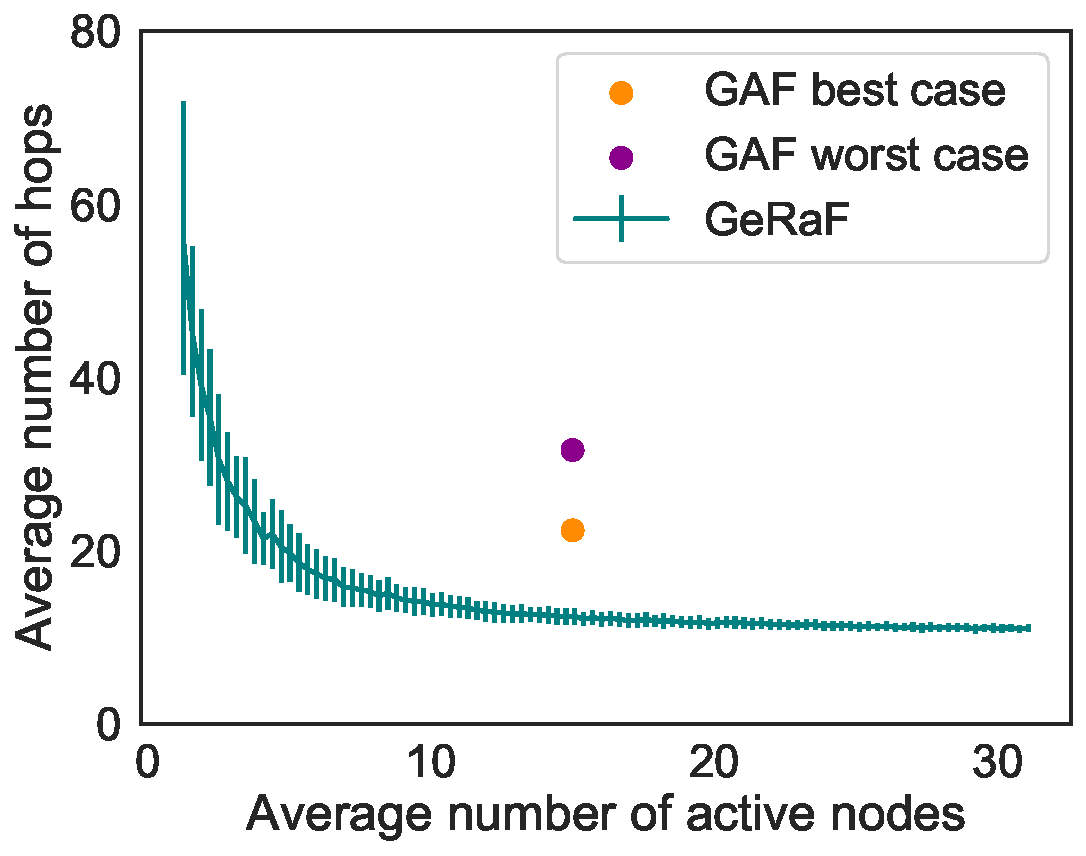
\includegraphics[width=\textwidth]{../multihop_GeRaF/figures/multihop_GeRaF_N100_distance10.pdf}
         \caption{Average number of hops vs average number of active nodes for $D=10$.}\label{fig:gaf10}
     \end{subfigure}
     
          \begin{subfigure}{0.5\textwidth}
         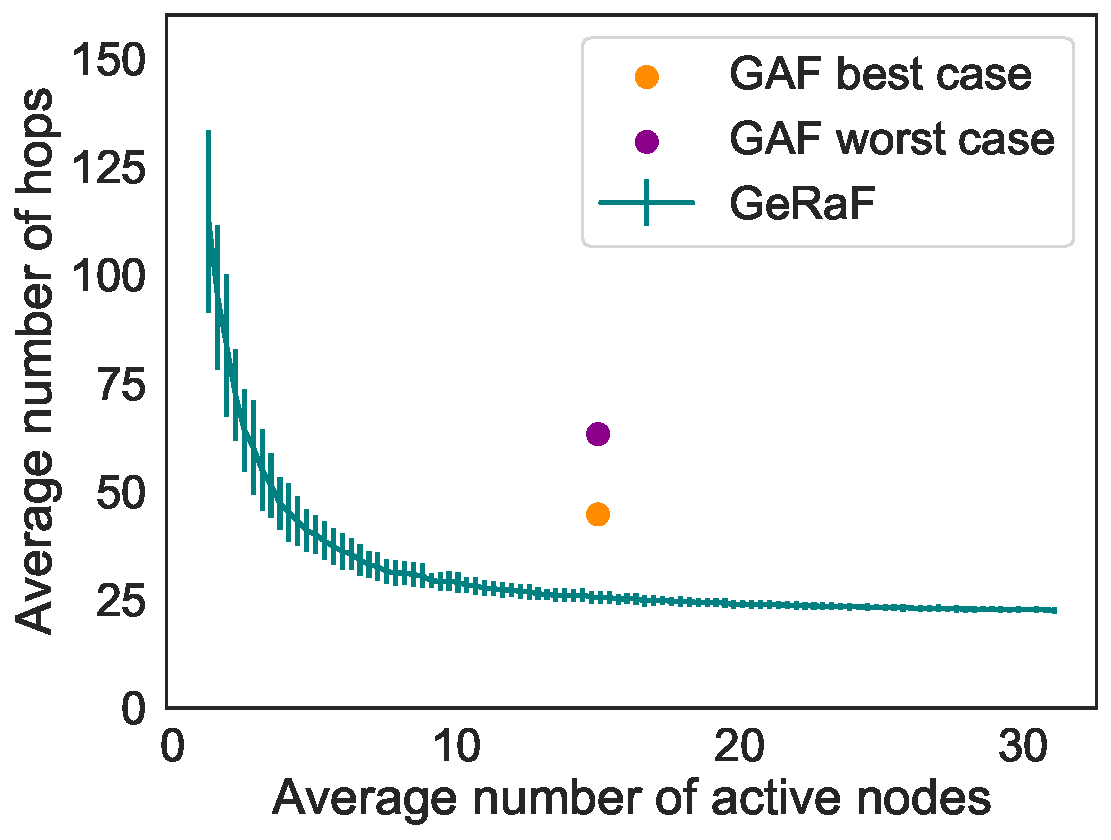
\includegraphics[width=\textwidth]{../multihop_GeRaF/figures/multihop_GeRaF_N100_distance20.pdf}
         \caption{Average number of hops vs average number of active nodes for $D=20$.}\label{fig:gaf20}
     \end{subfigure}
     
  \caption{Average number of hops and respective standard deviation vs average number of active nodes for different distances between sources and destination.}\label{fig:gaf}
\end{figure}


\bibliography{bib}

\end{document}

